\section{The Background Channels}\label{sec:bkg}
% The dominant SM backgrounds can be divided into two categories: (i) from leptonic $\tau$ decays and (ii) from fake leptons. In the first category, the dominant process is the pair production of $W Z$ with $W$ decaying leptonically and $Z \rightarrow \tau \tau$. The trilepton final states with no-OSSF pairs can arise from the subsequent leptonic decay of $\tau$ 's. We estimate this background process via Monte Carlo simulations.
% \\
% The dominant processes of the second category are $\gamma^{*} / Z+$ jets and $t \bar{t}$, where two leptons come from $\gamma^{*} / Z \rightarrow \tau \tau$ or the prompt decay of $t$ and $\bar{t}$, and a third lepton is faked from jets containing heavy-flavor mesons.
We define background as anything that is not of interest and that mimics the signals of new physics considered. 
As will be further explained in  later sections, we will explicitly demand a 3-lepton final-state in all collisions 
considered in the analysis. This will remove a lot of background, but not all. Due to the imperfect nature of the 
reconstruction of events, a demand for 3-lepton final-state will not be without errors. This leaves room for more 
variation in the background than one might expect. In this section I will cover the channels\footnote{By channels,
we refer to the physical diversity which could lead to a specific final-state. Often this refers to 
the different particles which mediates the process from initial- to final-state.} which will 
be of importance during the analysis. I will also discuss which background channels are the hardest 
to reduce in a potential new physics signal region, also called the irreducible background. These are 
channels that exhibit similar trends/distribution in the features. Note that the sections bellow
are listed by contribution to the 3-lepton final-state data (from most to least).  

\subsection{Z-jets}
The Z-jets channel is the largest contribution in all the data. The channel consists of all events
resulting in a Z-boson alongside jets. In the cases the Z-boson decays into two leptons, the additional 
jet acts as a fake lepton and the channel classifies as a 3-lepton final state. In figure \ref{fig:z_pjets} 
I have written the Feynman diagram of an example of such a channel. The figure shows a quark-antiquark leading 
to a Z-boson and gluon. The Z boson decays into two leptons (normally 
$e^-e^+$ or $\mu^- \mu^+$) and the gluon hadronises as a jet of hadrons which may obtain a b-hadron leading to a 
fake lepton. 

\subsection{Diboson (lll)}
Dibson channels are defined as channels resulting in two bosons. In the case of (lll), the dibosons
decay into a total of three leptons. In figure \ref{fig:wz} I have drawn the Feynman diagram of an 
example of such a channel. The figure shows a W- and Z-boson production through a quark-antiquark pair.
third quark. The W-boson decays into a lepton with missing energy\footnote{Neutrinos very rarely interact
with anything, making them almost impossible to detect. We therefore refer to neutrinos as missing energy.}
and the Z-boson decays into a pair of leptons. 

\subsection{$t\bar{t}$}
The $t\bar{t}$ channel is defined as a proton-proton collision resulting in a pair of top quark-antiquark. 
In figure \ref{fig:ttbar} I have drawn a Feynman diagram of an example of such a channel. The figure 
shows gluon-gluon fusion producing a pair of top quarks. The top-antitop pair decay into a bottom-quark 
and a W boson. The channel constitutes a background when both W bosons decay into a charged and a neutral 
lepton and one of the b-quarks leads to a fake lepton.

\subsection{Diboson (llll)}
In the case of diboson (llll), the channel refers to events resulting in two Z-bosons which decay 
into four leptons. In figure \ref{fig:zz} I have drawn a Feynman diagram of an example of 
such a diagram. The figure shows a quark-antiquark pair annihilating into two Z-bosons.
The two Z-bosons decay into two pairs of leptons. This process constitutes a backgorund when one 
of the leptons is not reconstructed in the detector.


\subsection{Top Others}
\subsection{Single Others}
\subsection{Diboson (ll)}
\subsection{Others}


\begin{figure}
    \centering
    \vfill
    \makebox[\linewidth][c]{%
    \begin{subfigure}{.5\textwidth}
        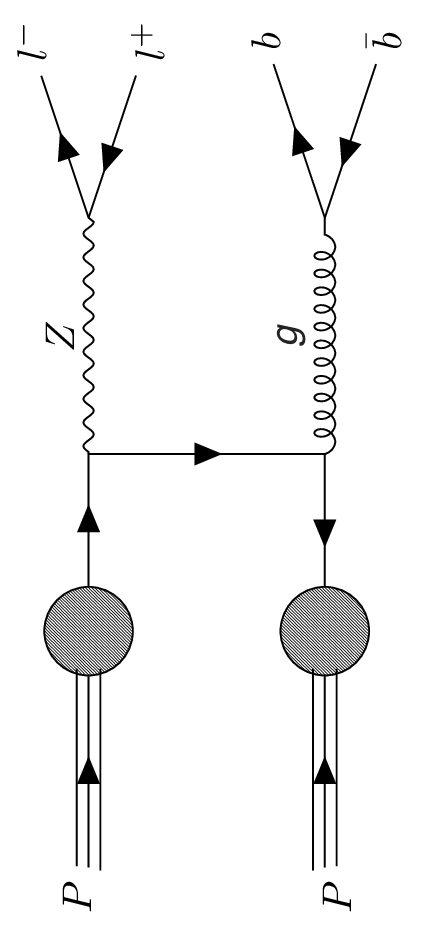
\includegraphics[width=0.45\textwidth, angle = -90]{Figures/FDiagrams/Z_pjets.png}
        \caption{}
        \label{fig:z_pjets}
    \end{subfigure}
    \hspace{1.5cm}
    \begin{subfigure}{.5\textwidth}
        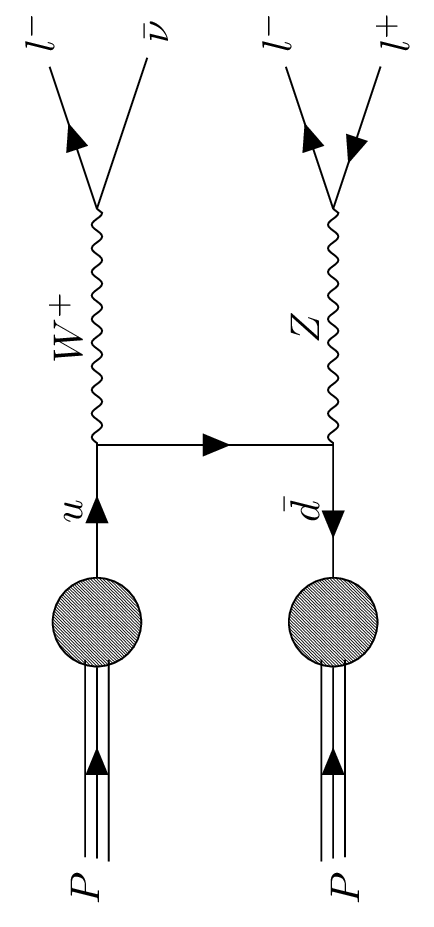
\includegraphics[width=0.45\textwidth, angle = -90]{Figures/FDiagrams/wz.png}
        \caption{}
        \label{fig:wz}
    \end{subfigure}
    }
    \vfill
    \makebox[\linewidth][c]{%
    \begin{subfigure}{.5\textwidth}
        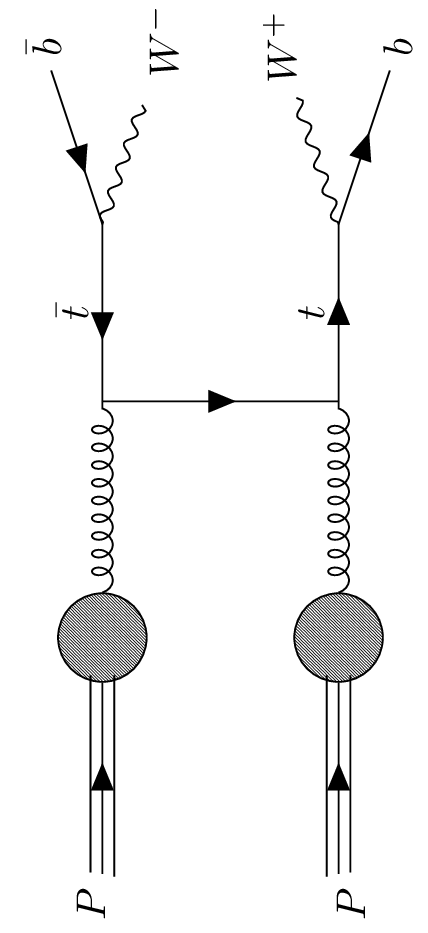
\includegraphics[width=0.45\textwidth, angle = -90]{Figures/FDiagrams/ttbar.png}
        \caption{}
        \label{fig:ttbar}
    \end{subfigure}
    \hspace{1.5cm}
    \begin{subfigure}{.5\textwidth}
        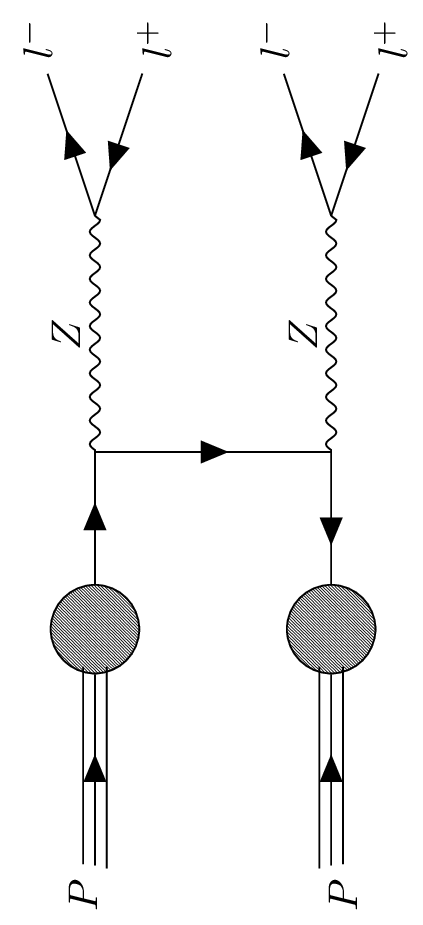
\includegraphics[width=0.45\textwidth, angle = -90]{Figures/FDiagrams/zz.png}
        \caption{}
        \label{fig:zz}
    \end{subfigure}
    }
    \vfill
    \makebox[\linewidth][c]{%
    \begin{subfigure}{.5\textwidth}
        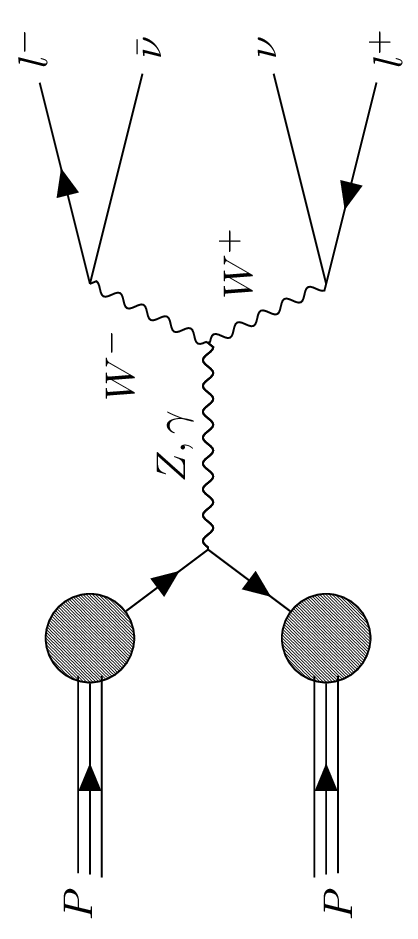
\includegraphics[width=0.45\textwidth, angle = -90]{Figures/FDiagrams/ww.png}
        \caption{}
        \label{fig:ww}
    \end{subfigure}
    \hspace{1.5cm}
    \begin{subfigure}{.5\textwidth}
        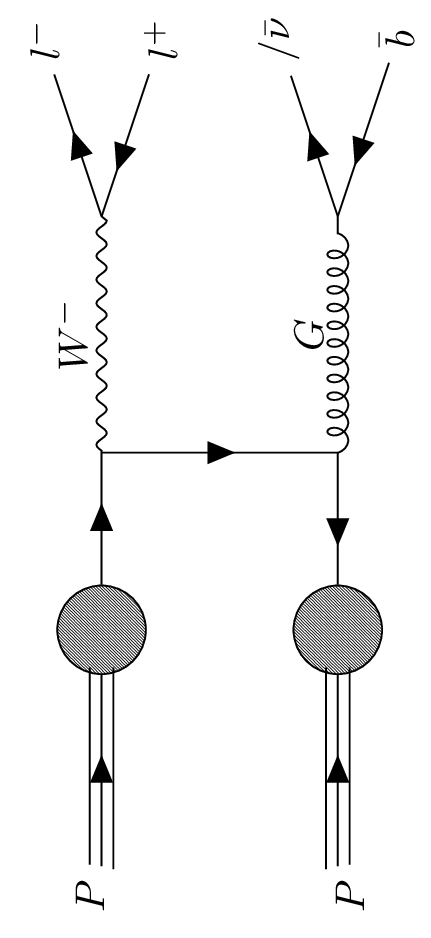
\includegraphics[width=0.45\textwidth, angle = -90]{Figures/FDiagrams/w_pjets.png}
        \caption{}
        \label{fig:w_pjets}
    \end{subfigure}
    }
    \makebox[\linewidth][c]{%
    \begin{subfigure}{.5\textwidth}
        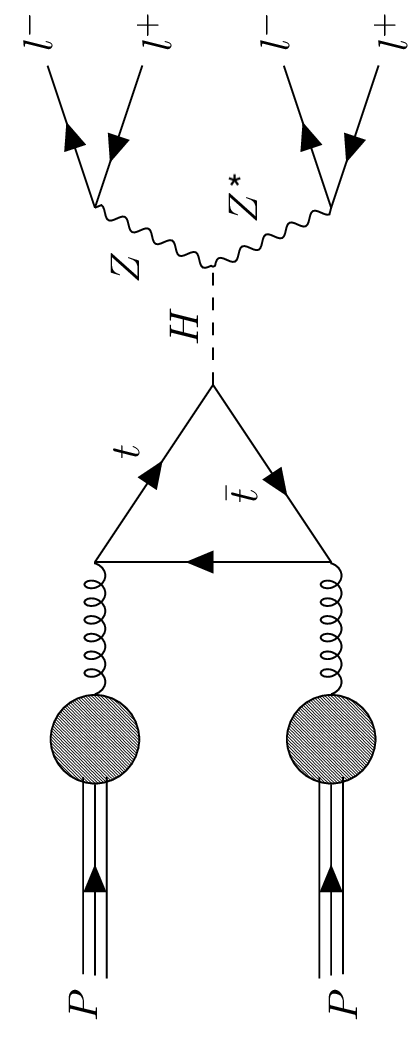
\includegraphics[width=0.45\textwidth, angle = -90]{Figures/FDiagrams/h.png}
        \caption{}
        \label{fig:h}
    \end{subfigure}
    \hspace{1.5cm}
    \begin{subfigure}{.5\textwidth}
        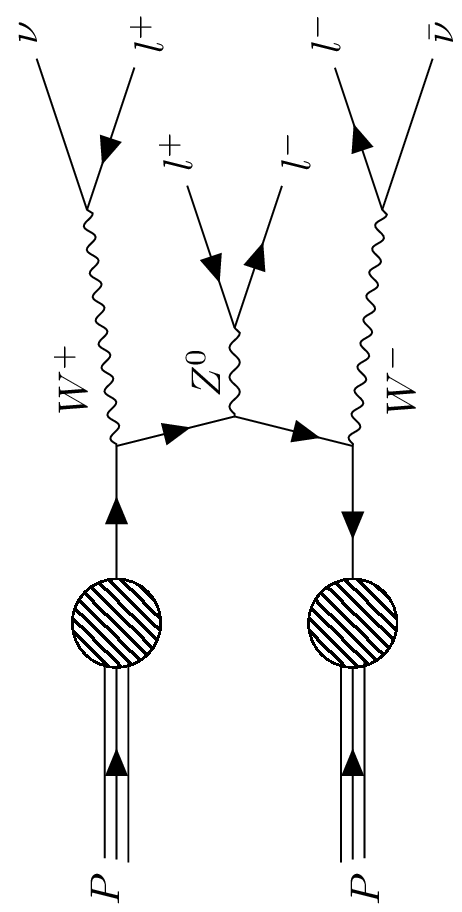
\includegraphics[width=0.46\textwidth, angle = -90]{Figures/FDiagrams/WZW.png}
        \caption{}
        \label{fig:zzz}
    \end{subfigure}
    }
    \caption{}
    \label{fig:Feynman}
\end{figure}
\newpage
